\section{Results}


\begin{frame}{Test Problem: Lorenz96}
We test the Lorenz96 ODE:
$$\dot{x}_i = (x_{i+1} - x_{i-2})x_{i-1} - x_i + F,$$
and take the initial condition randomly generated in the cube $[-5, 5]^d$, and randomly generate $F \in [1,5]$.

\begin{center}
    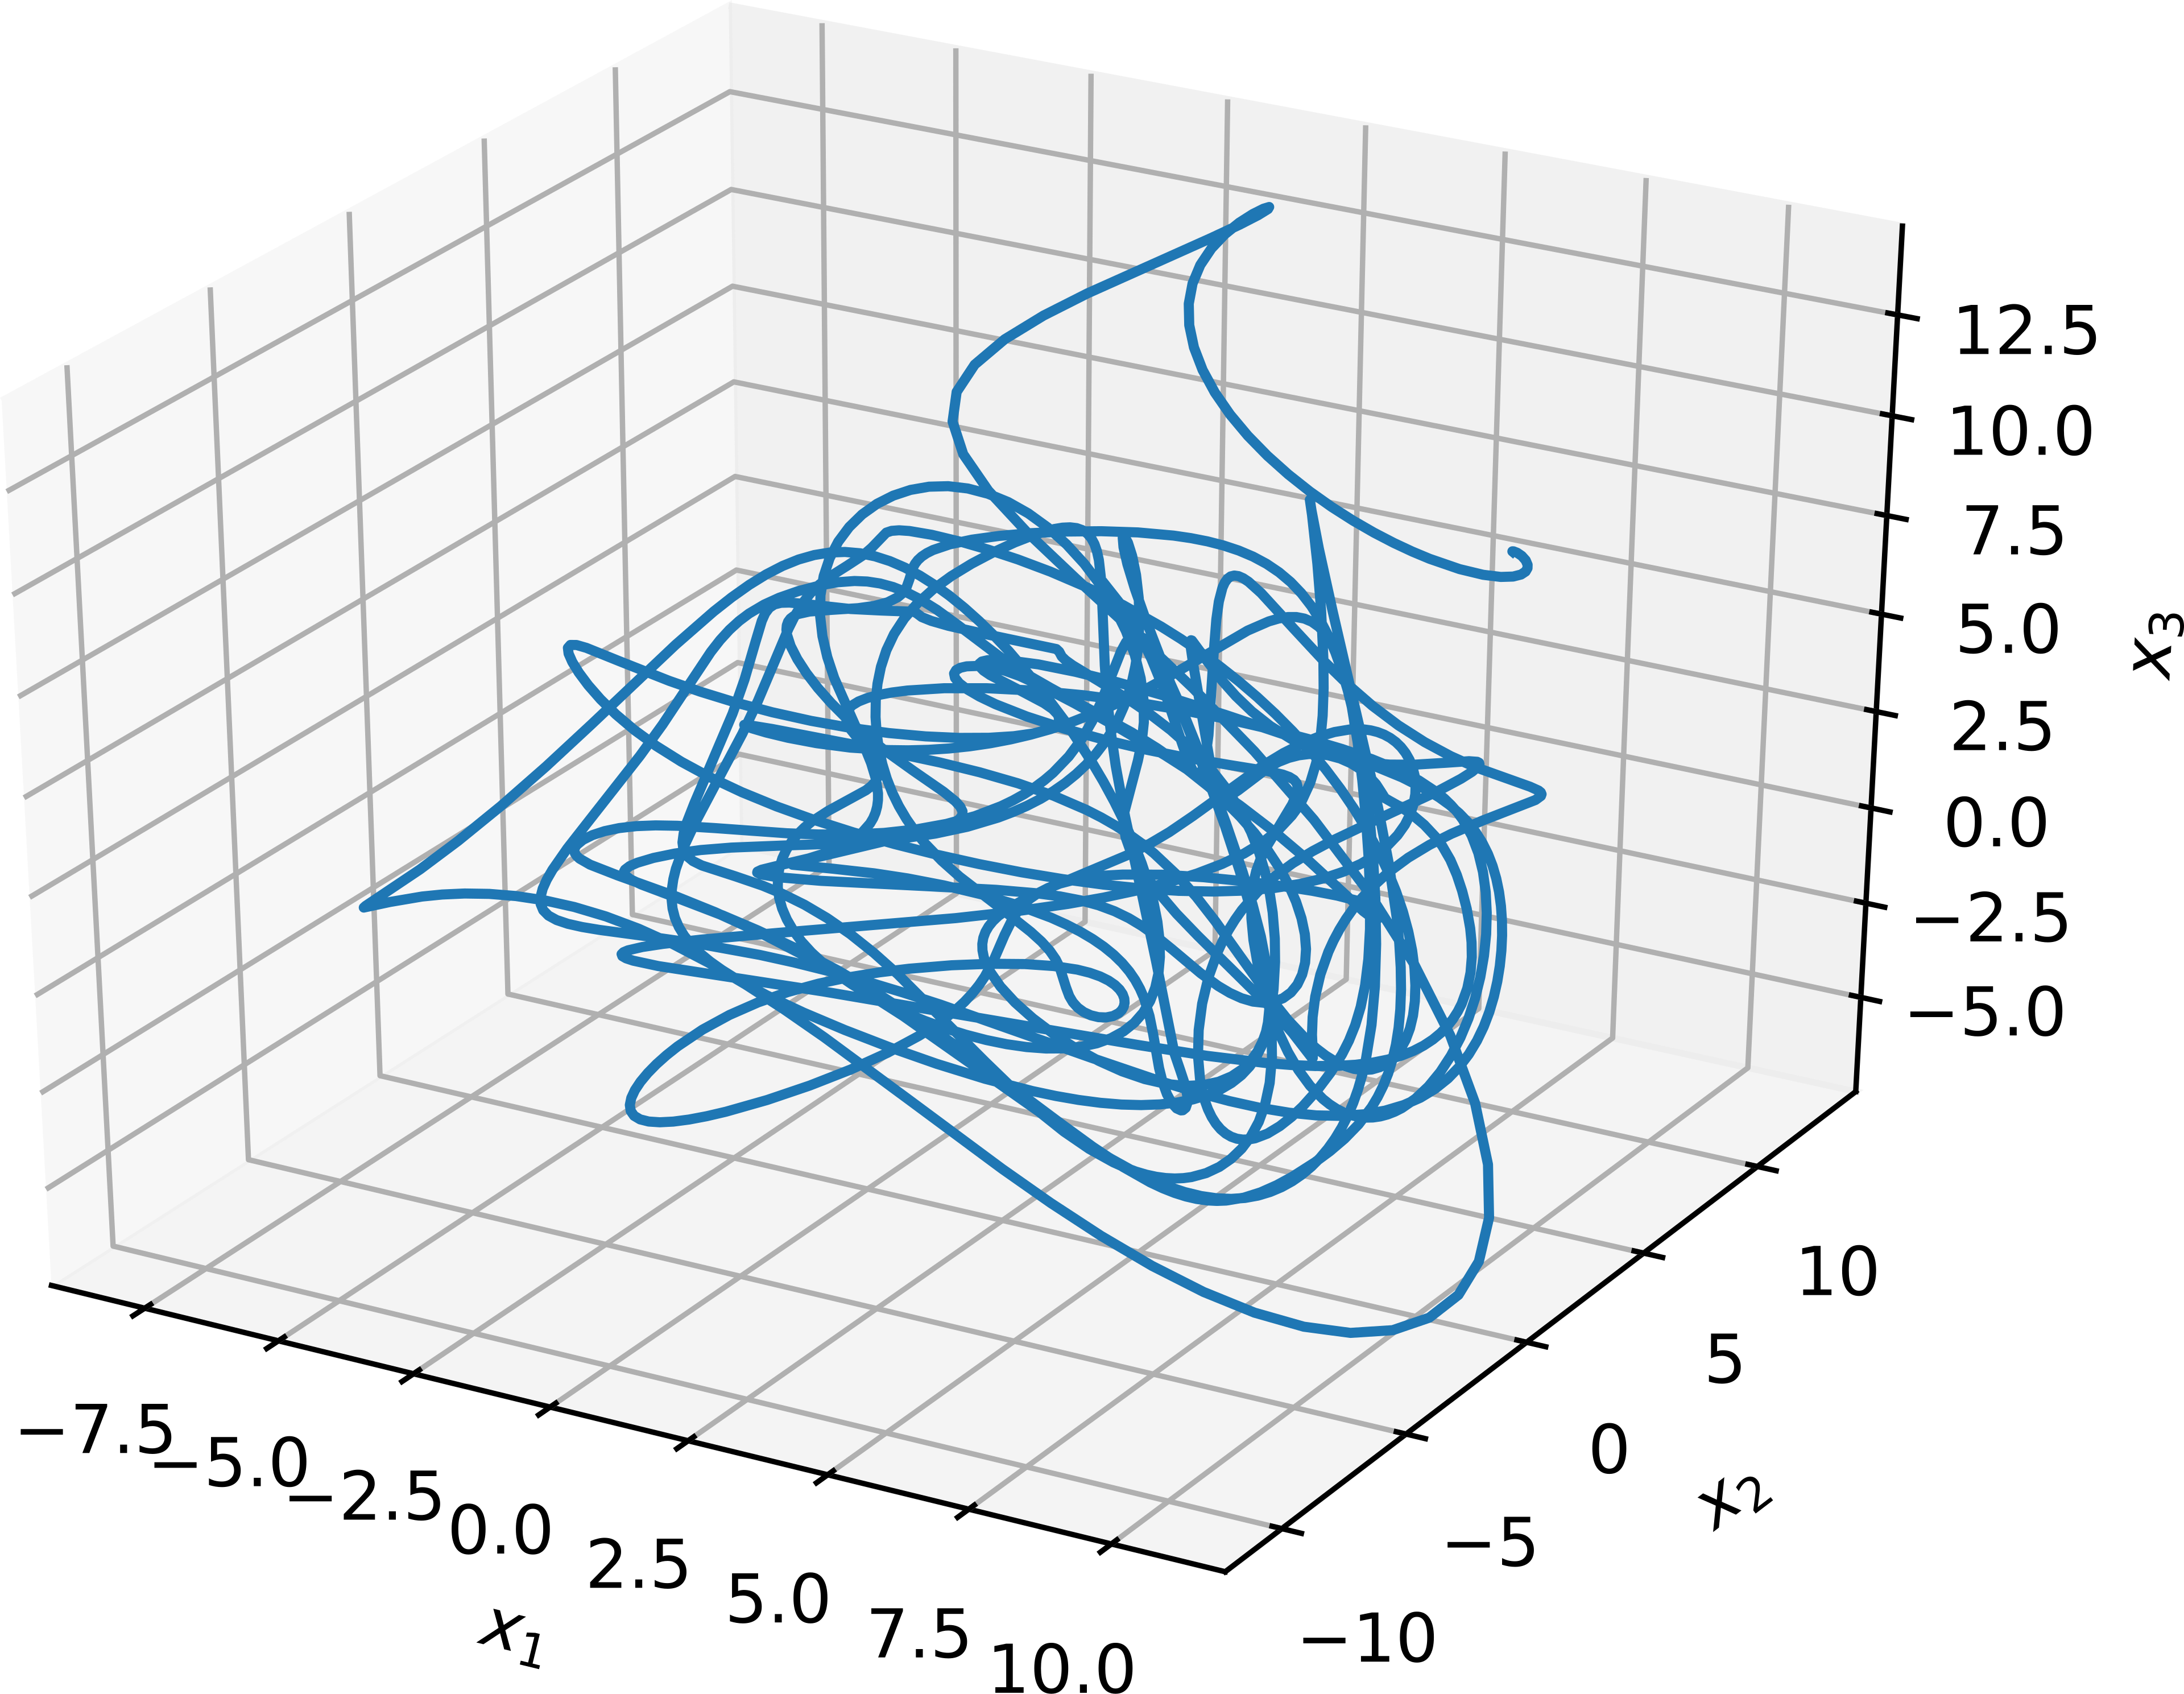
\includegraphics[width=0.4\linewidth]{../figs/Lorenz_96.svg.png}
\end{center}

\end{frame}

\begin{frame}{Comparing Time-Stepping}
Compare two different compute kernels:
\begin{itemize}
    \item \texttt{forward\_euler\_kernel}: on one thread, takes a single time step. Measure time for steps taken until completion.
    \item \texttt{forward\_euler\_kernel\_multistep}: on one thread, runs a single IVP to completion. Measure time for a single launch
\end{itemize}
\begin{center}
    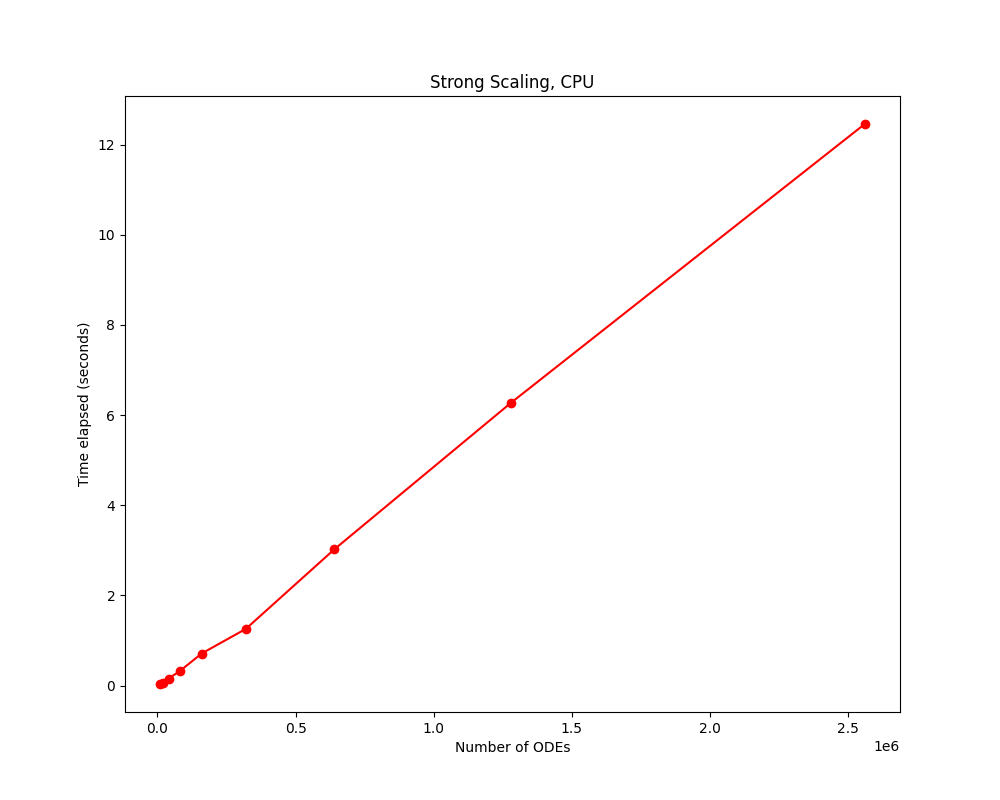
\includegraphics[width=0.4\linewidth]{../figs/strong_scaling_forward_euler_cpu.png} 
    \qquad 
    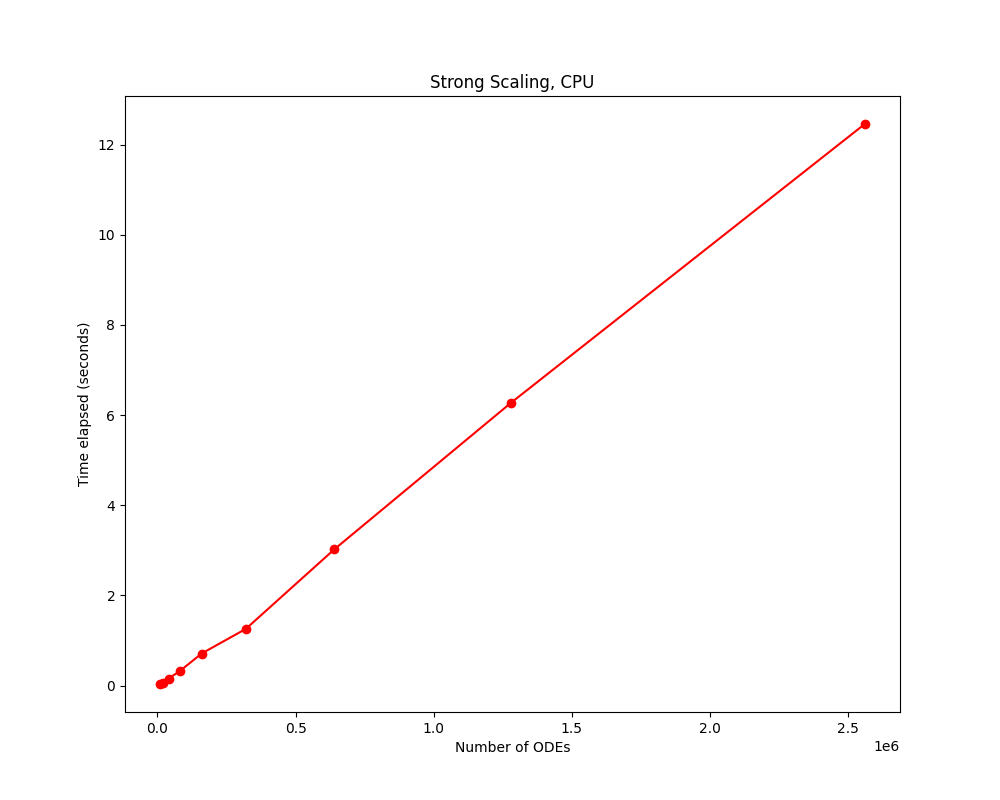
\includegraphics[width=0.4\linewidth]{../figs/strong_scaling_forward_euler_cpu.png} 
\end{center}
\end{frame}


\begin{frame}{Comparison to Serial Code}

\begin{tabular}{|c|c|c|c|}
\hline $N_{\mathrm{ode}}$ (x$10^6$) & Parallel Time (s) & Serial Time (s) & Speedup \\
\hline \\

\end{tabular}
    
\end{frame}


\begin{frame}{Next Steps}
\begin{itemize}
    \item Add load balancing.
    \begin{itemize}
        \item Idea: run for some number of time steps. Then rearrange data on the GPU so that faster ODEs relaunch on the same thread.
    \end{itemize}
    
    \item Add implicit time stepping.
    \begin{itemize}
        \item Solving nonlinear system of equations for each time step. Challenging to do per thread if $d$ is large.
    \end{itemize}

    \item Thank you!
\end{itemize}
\end{frame}
